% definicja rozmiaru czcionki oraz formatu strony
\documentclass[12pt,a4paper]{article} 
%\usepackage[letterpaper,top=2cm,bottom=2cm,left=3cm,right=3cm,marginparwidth=1.75cm]{geometry}


% Useful packages
% nagłowek dokumentu dzięki któremu użyjemy polskich znaków
\usepackage[utf8]{inputenc} 
\usepackage{amsmath, amsfonts, amssymb, polski, indentfirst, graphicx, enumerate}

\usepackage[colorlinks=true, allcolors=blue]{hyperref}

\title{GL03}
\author{w65550 - Piotr Najda}

\begin{document}
\maketitle

\section{Zadania podstawowe 1 - 4}

\begin{figure}[ht]
\centering
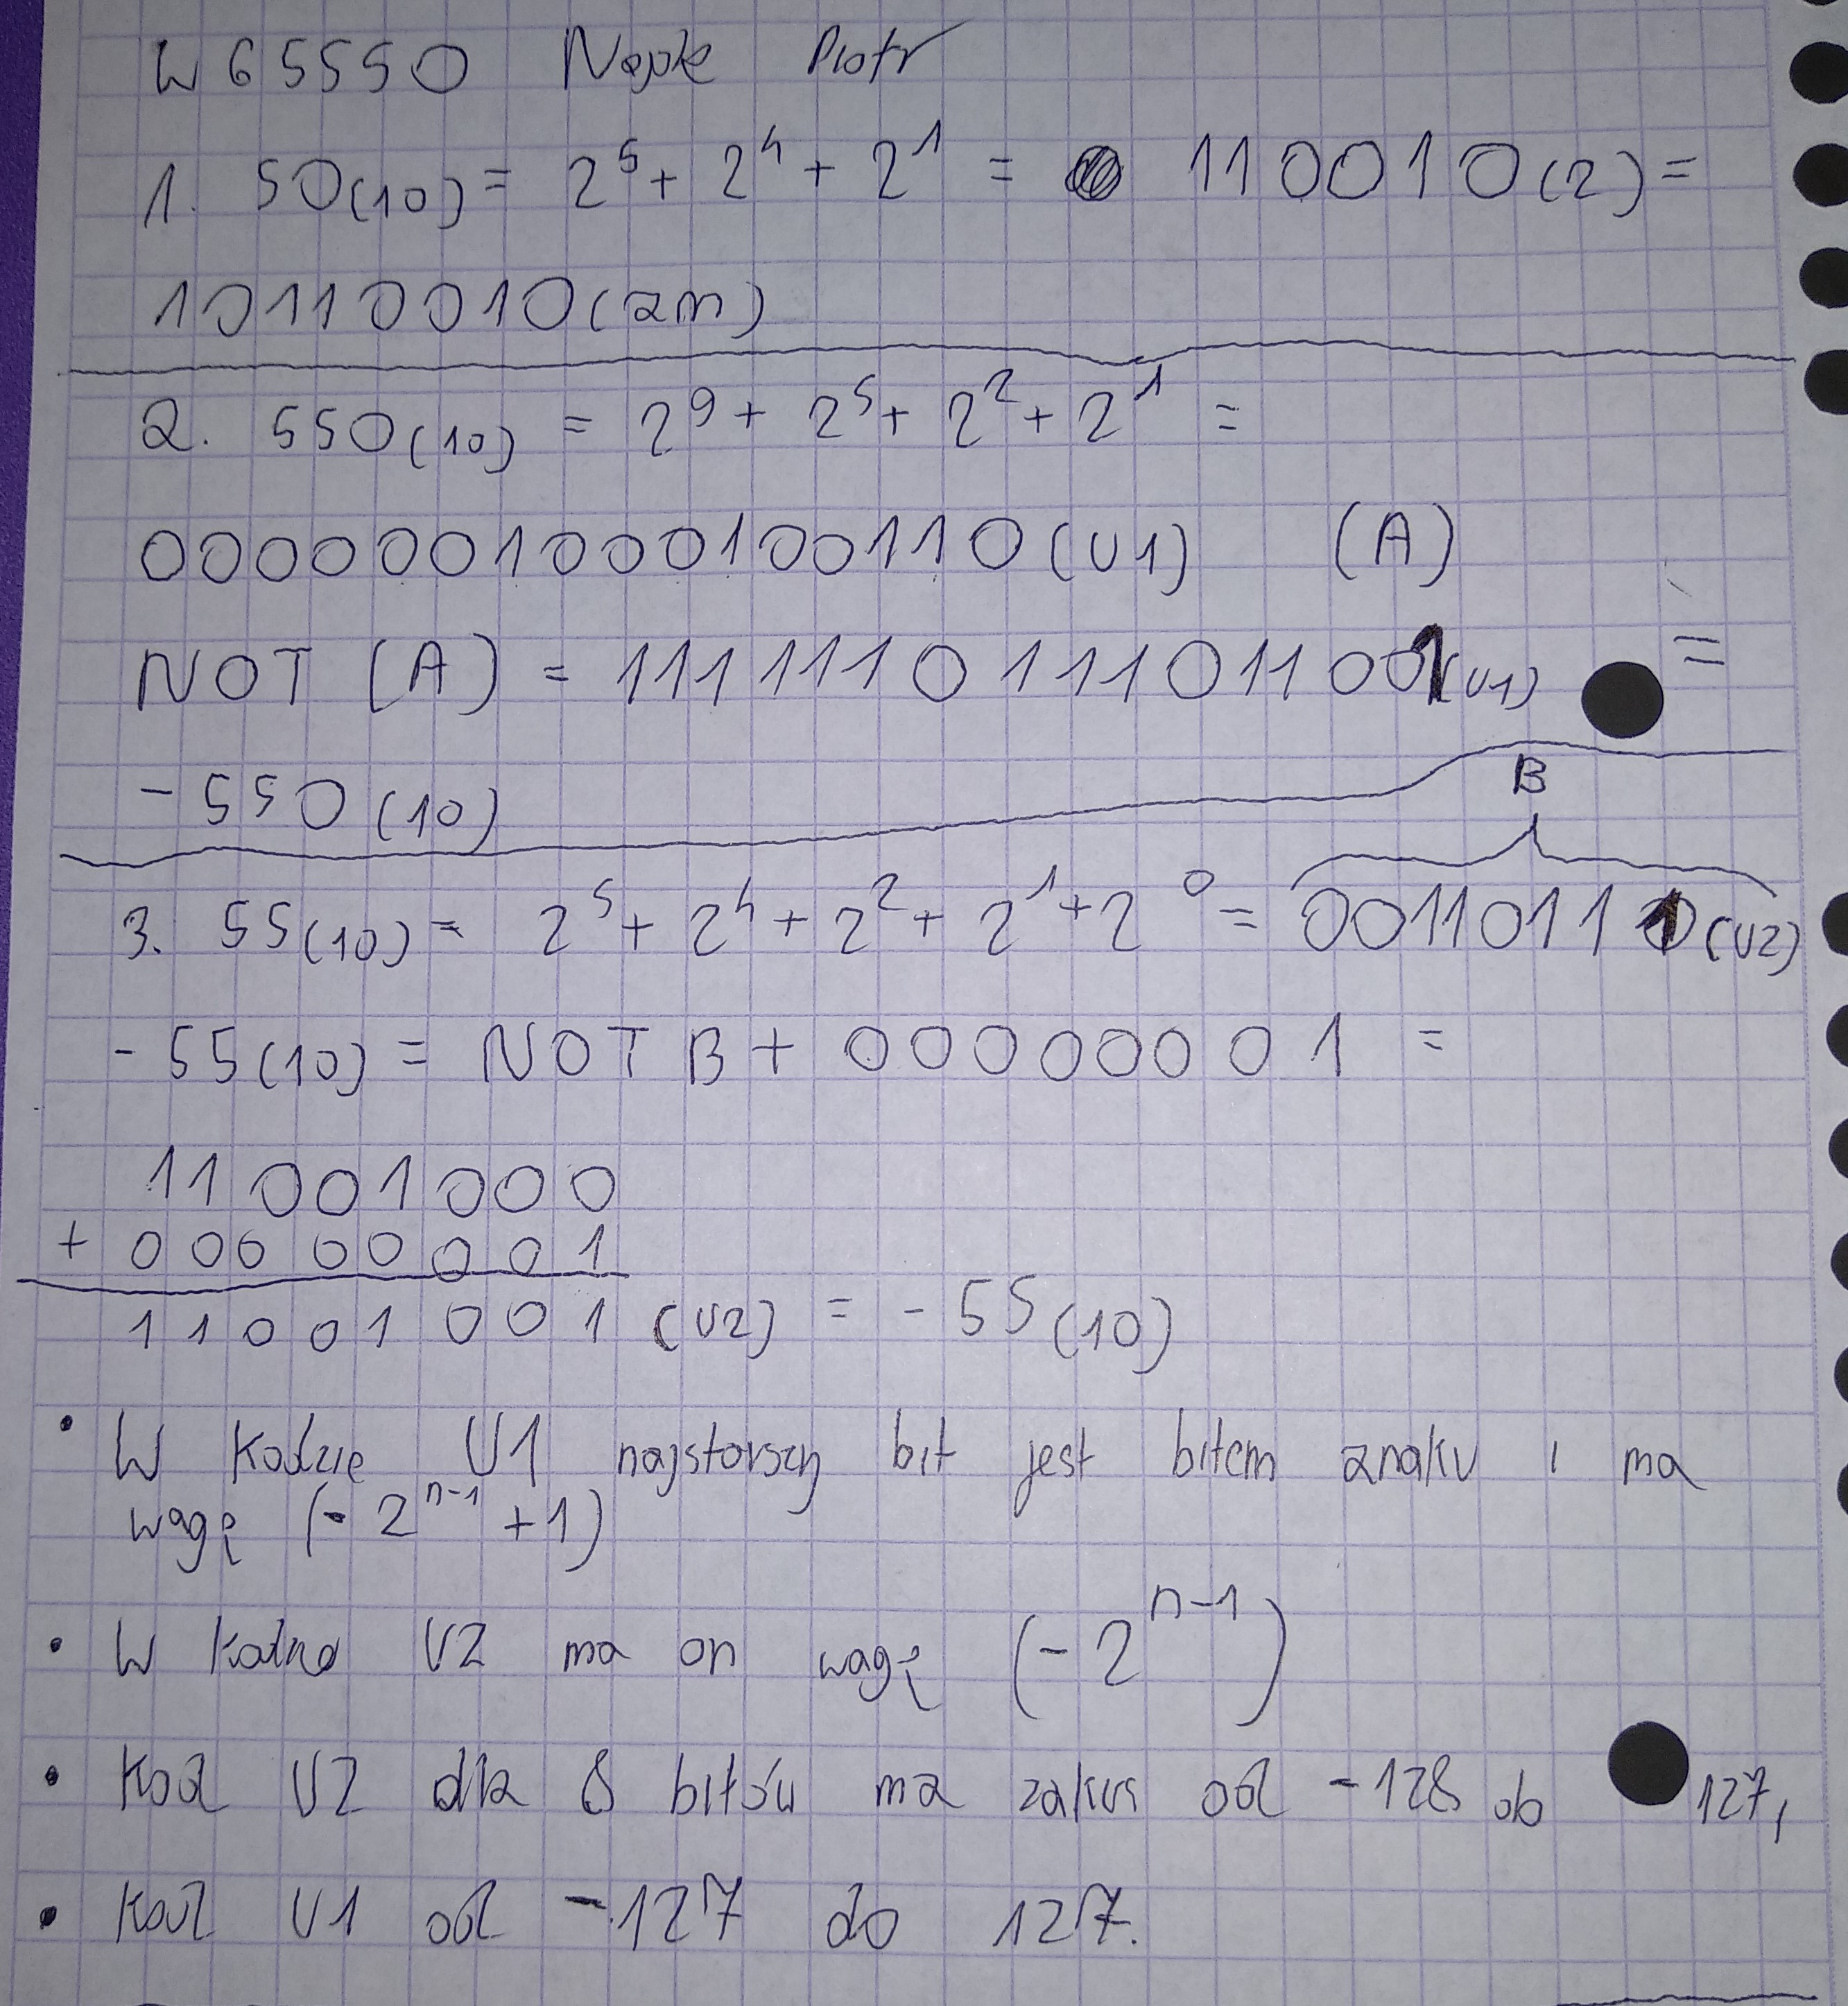
\includegraphics[width=0.80\textwidth]{IMG_20211102_174411.jpg}
\caption{\label{fig:zad1do3}Zadania 1 - 3}
\end{figure}

\begin{figure}[ht]
\centering
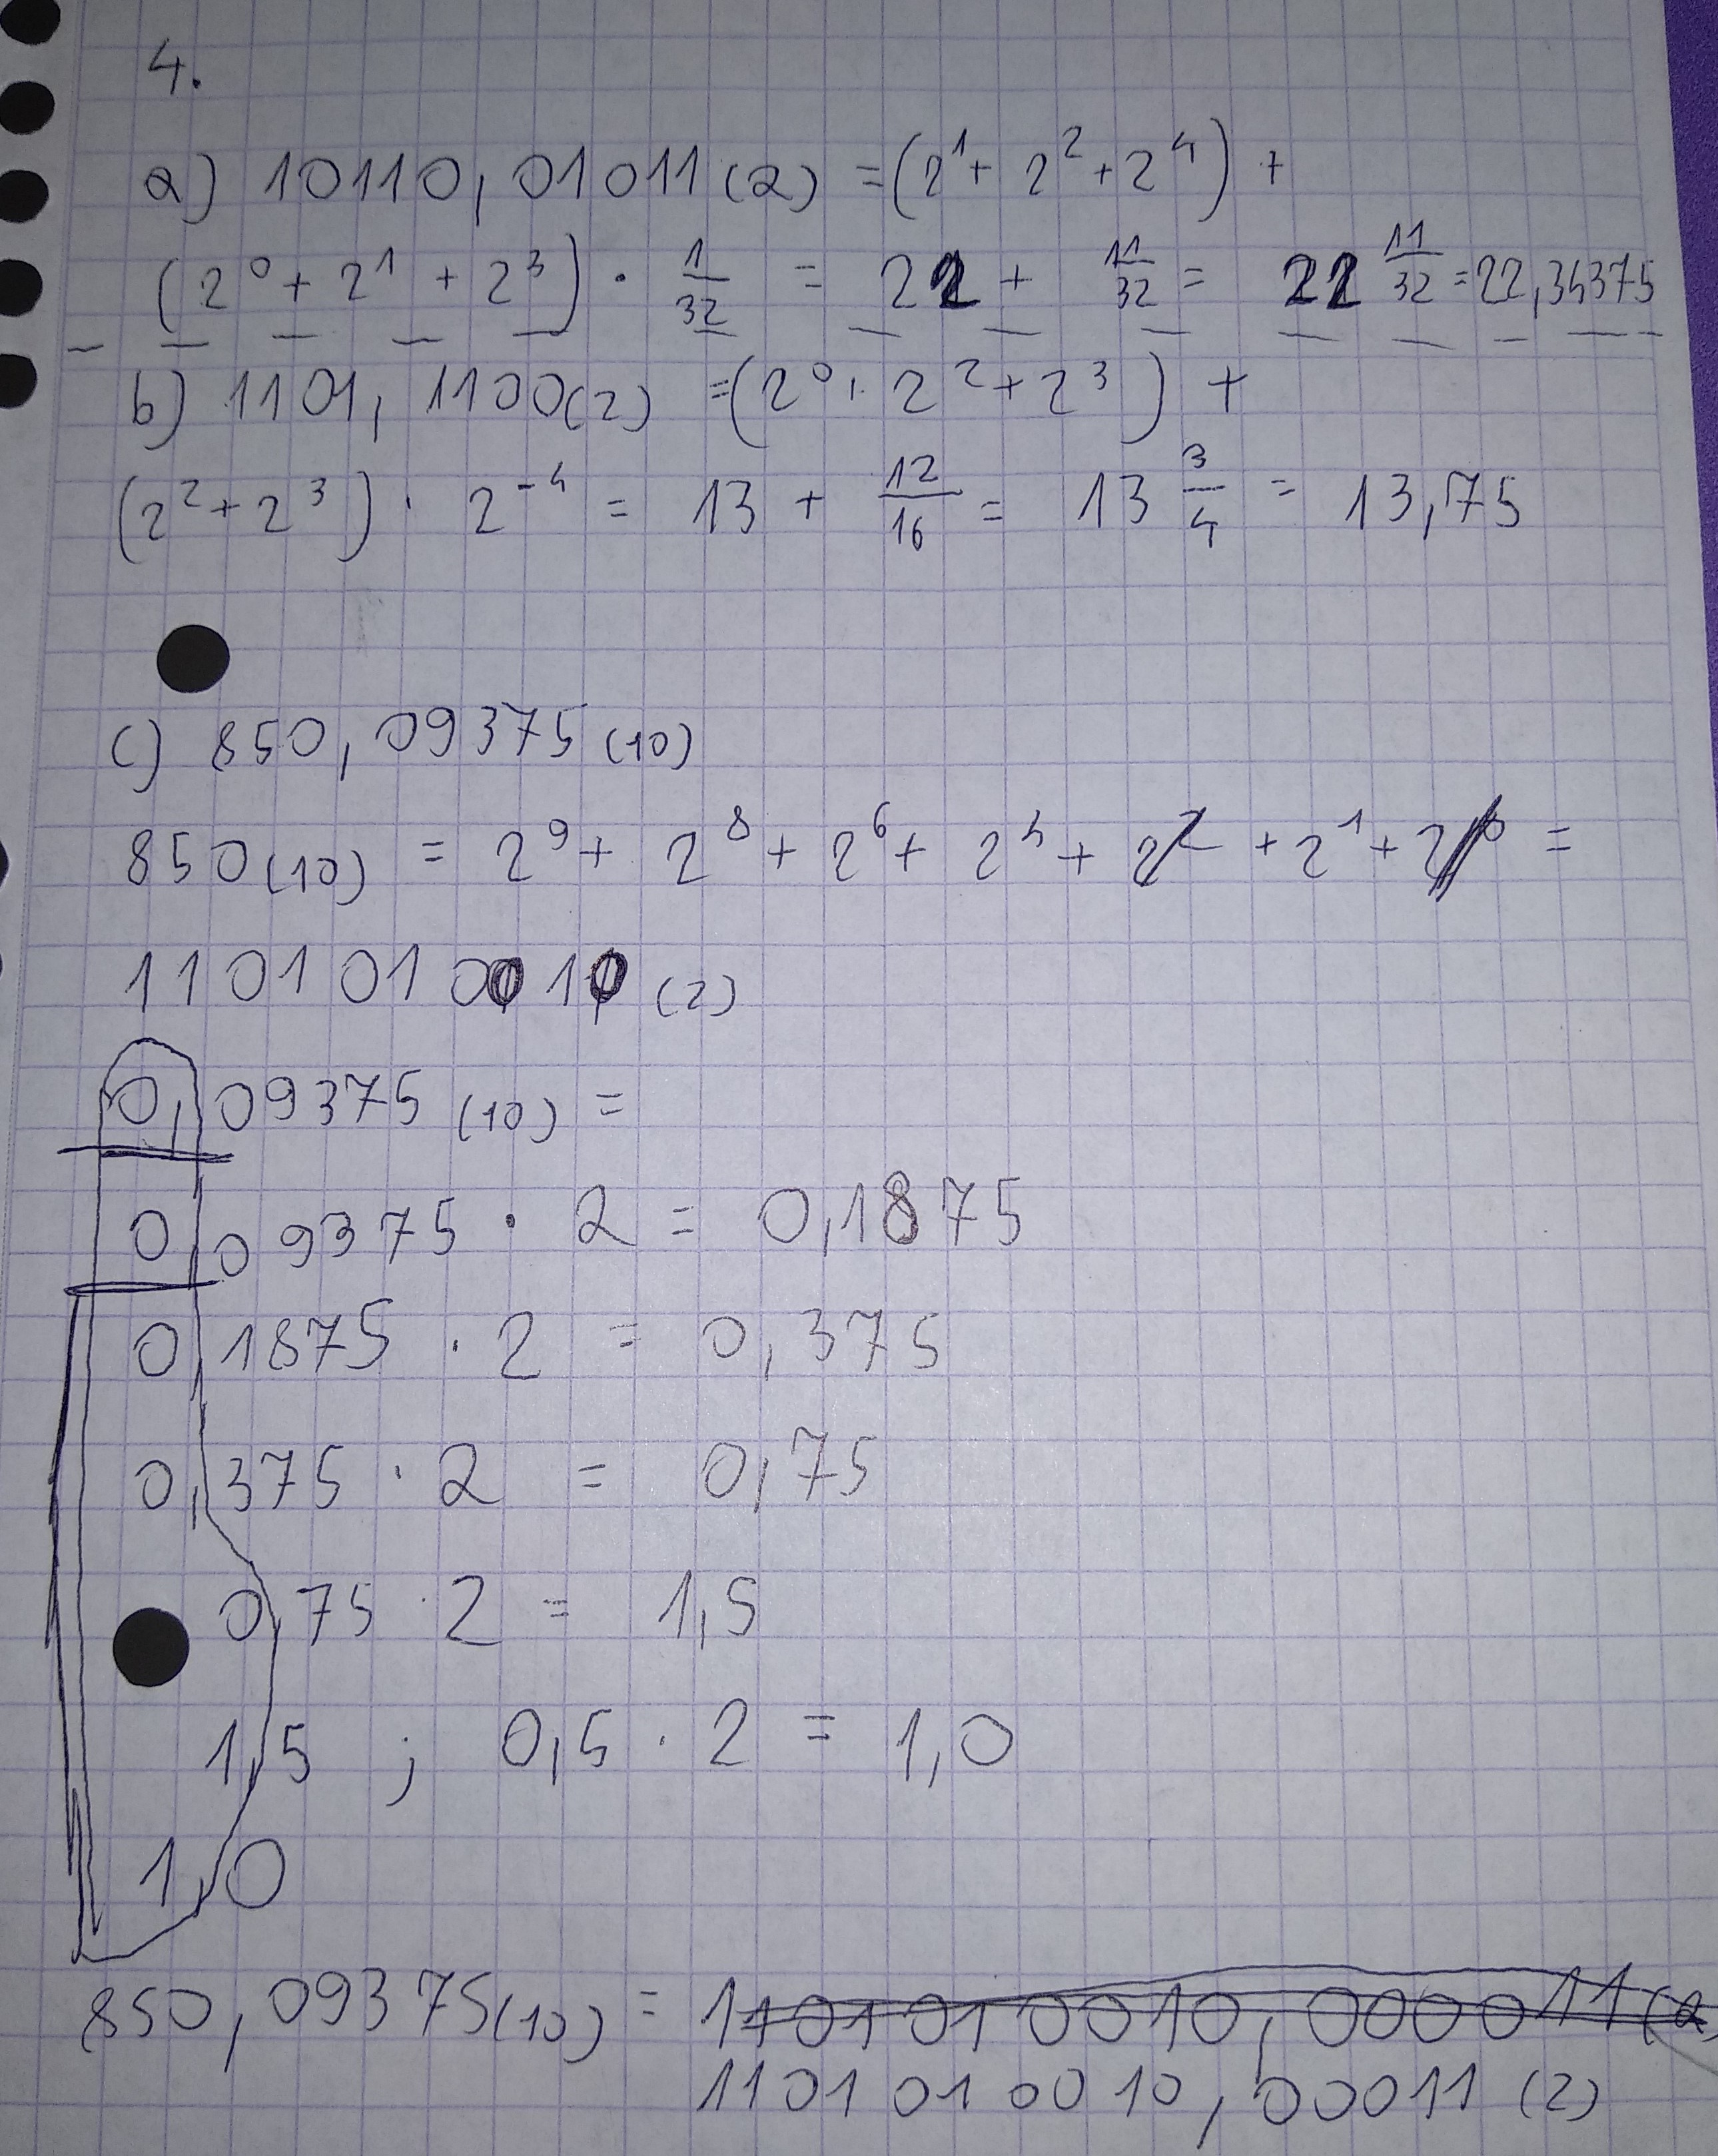
\includegraphics[width=0.75\textwidth]{IMG_20211102_174430~2.jpg}
\caption{\label{fig:zad4}Zadanie 4}
\end{figure}

\begin{figure}[ht]
\centering
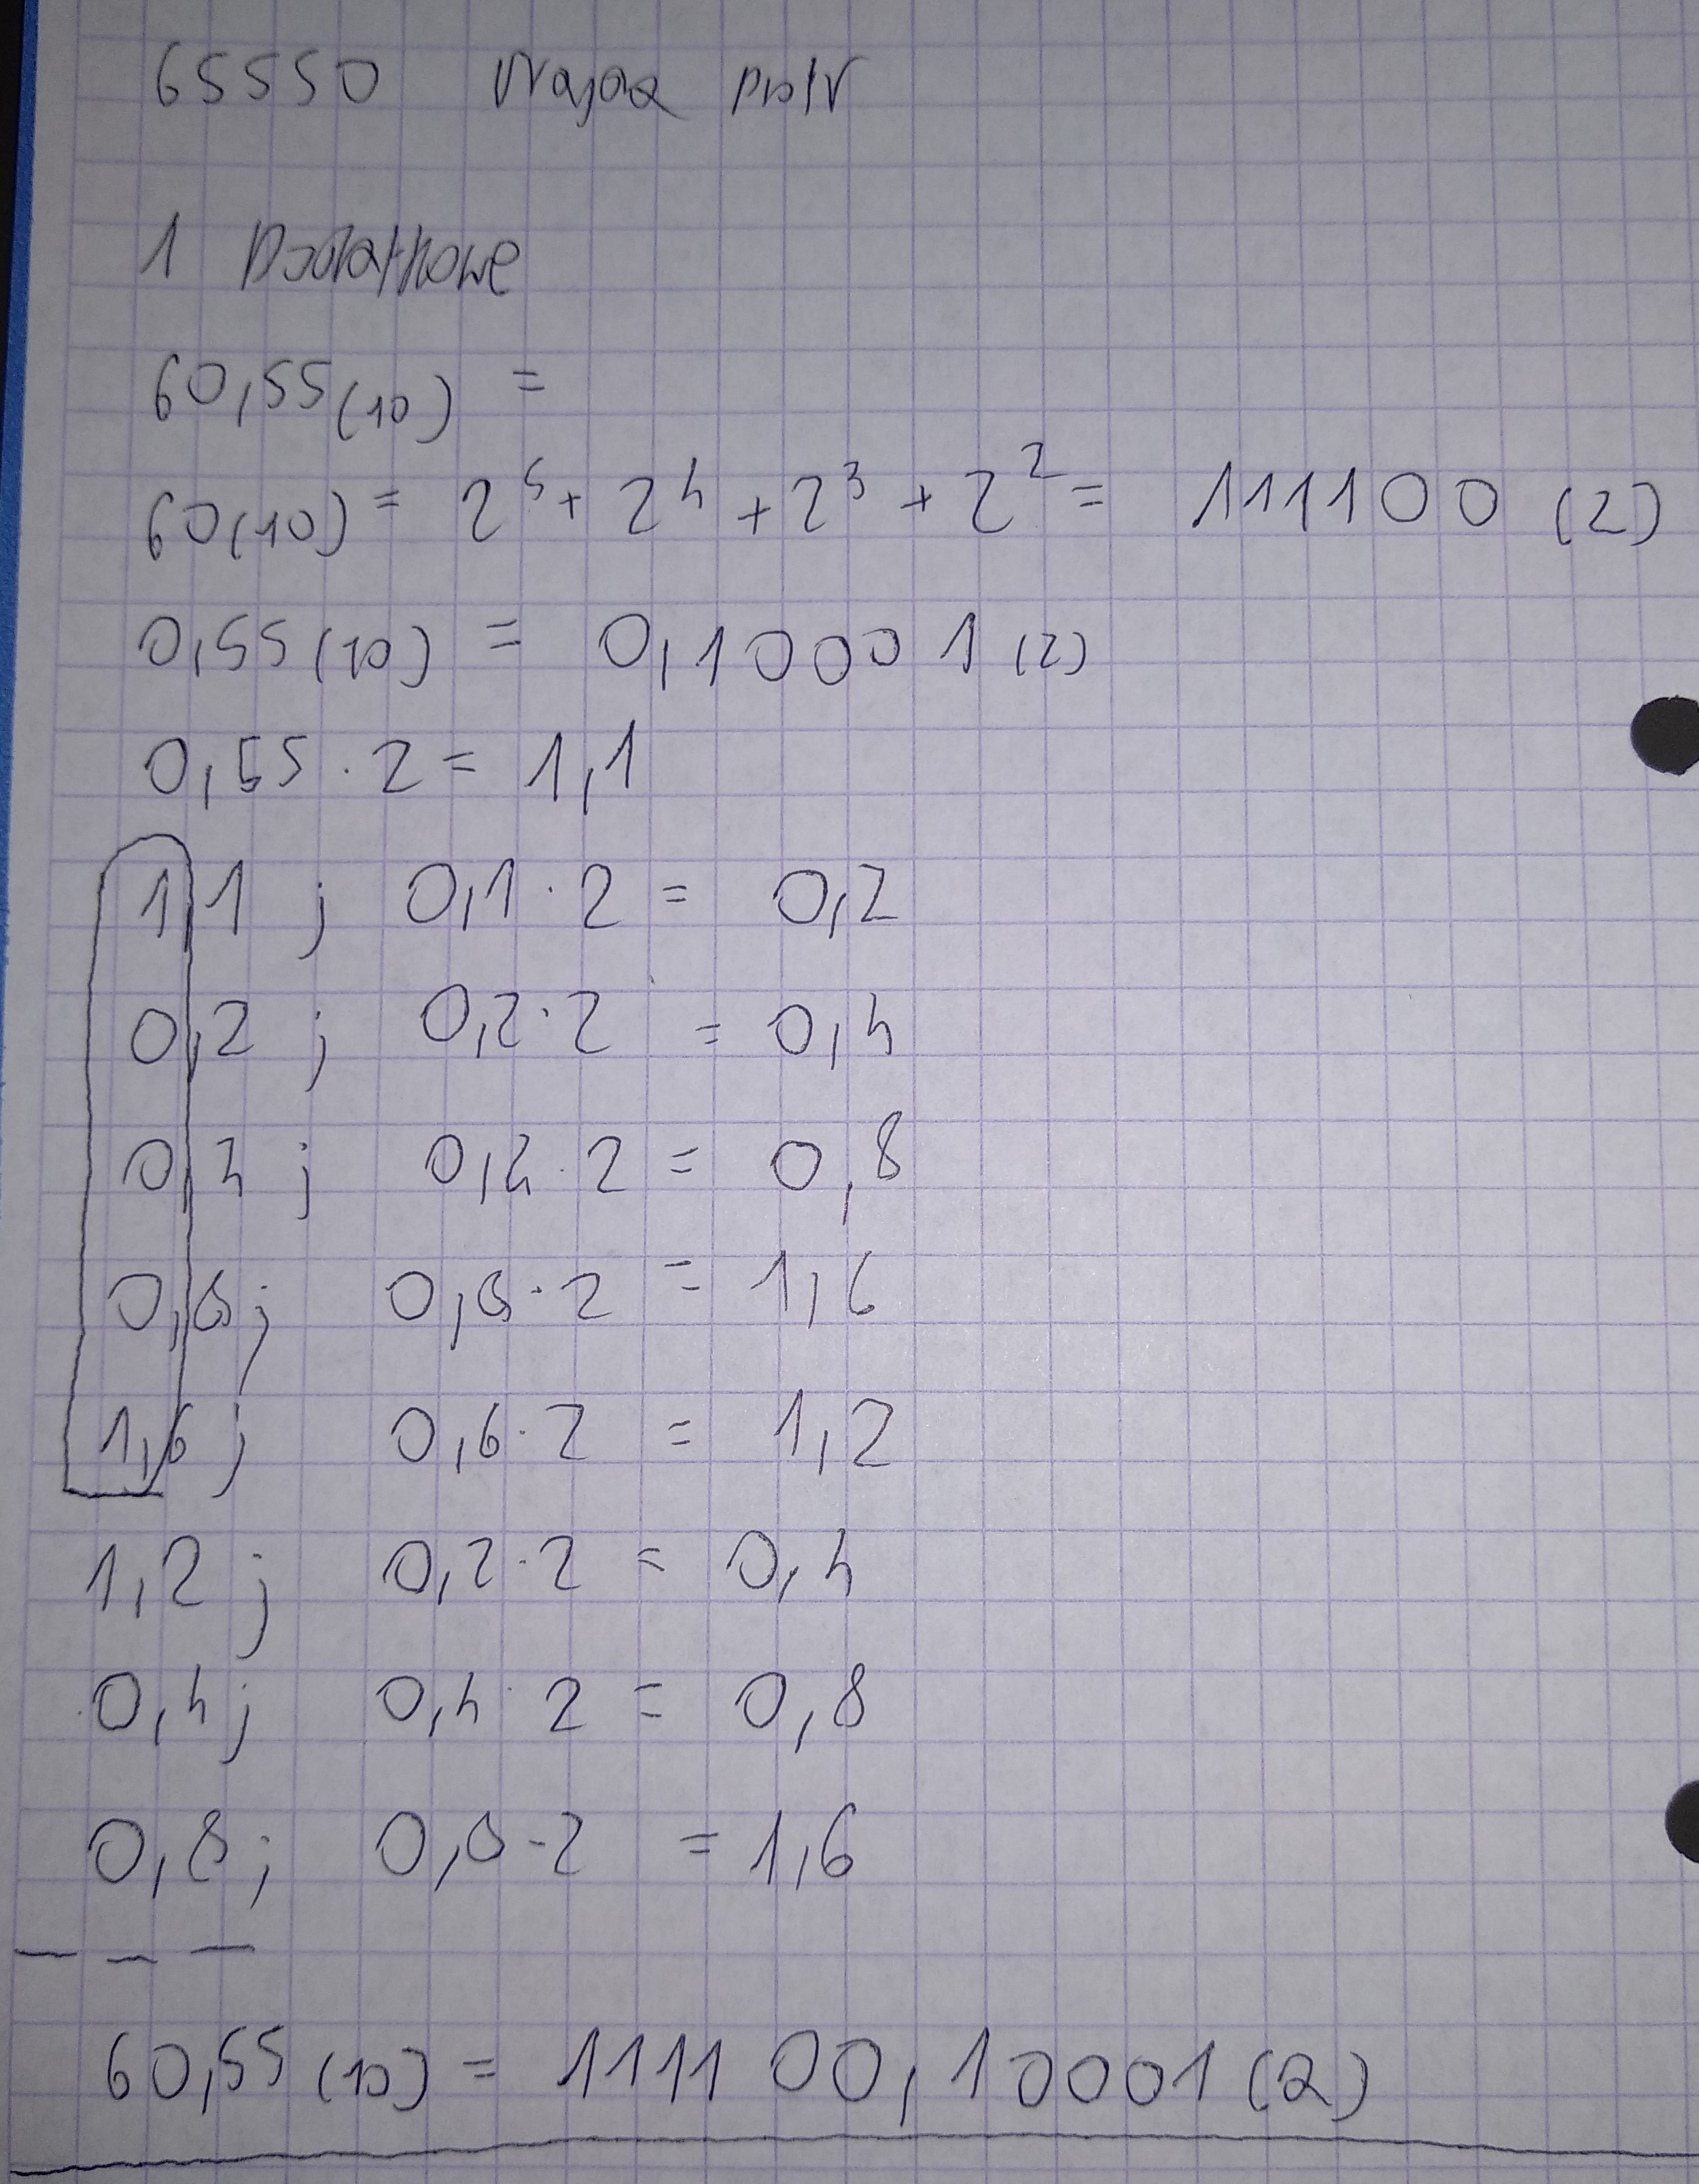
\includegraphics[width=0.9\textwidth]{IMG_20211102_174500~2.jpg}
\caption{\label{fig:zaddod1}Zadanie dodatkowe 1}
\end{figure}

\section{Zadania dodatkowe 1 - 2}

\begin{figure}[ht]
\centering
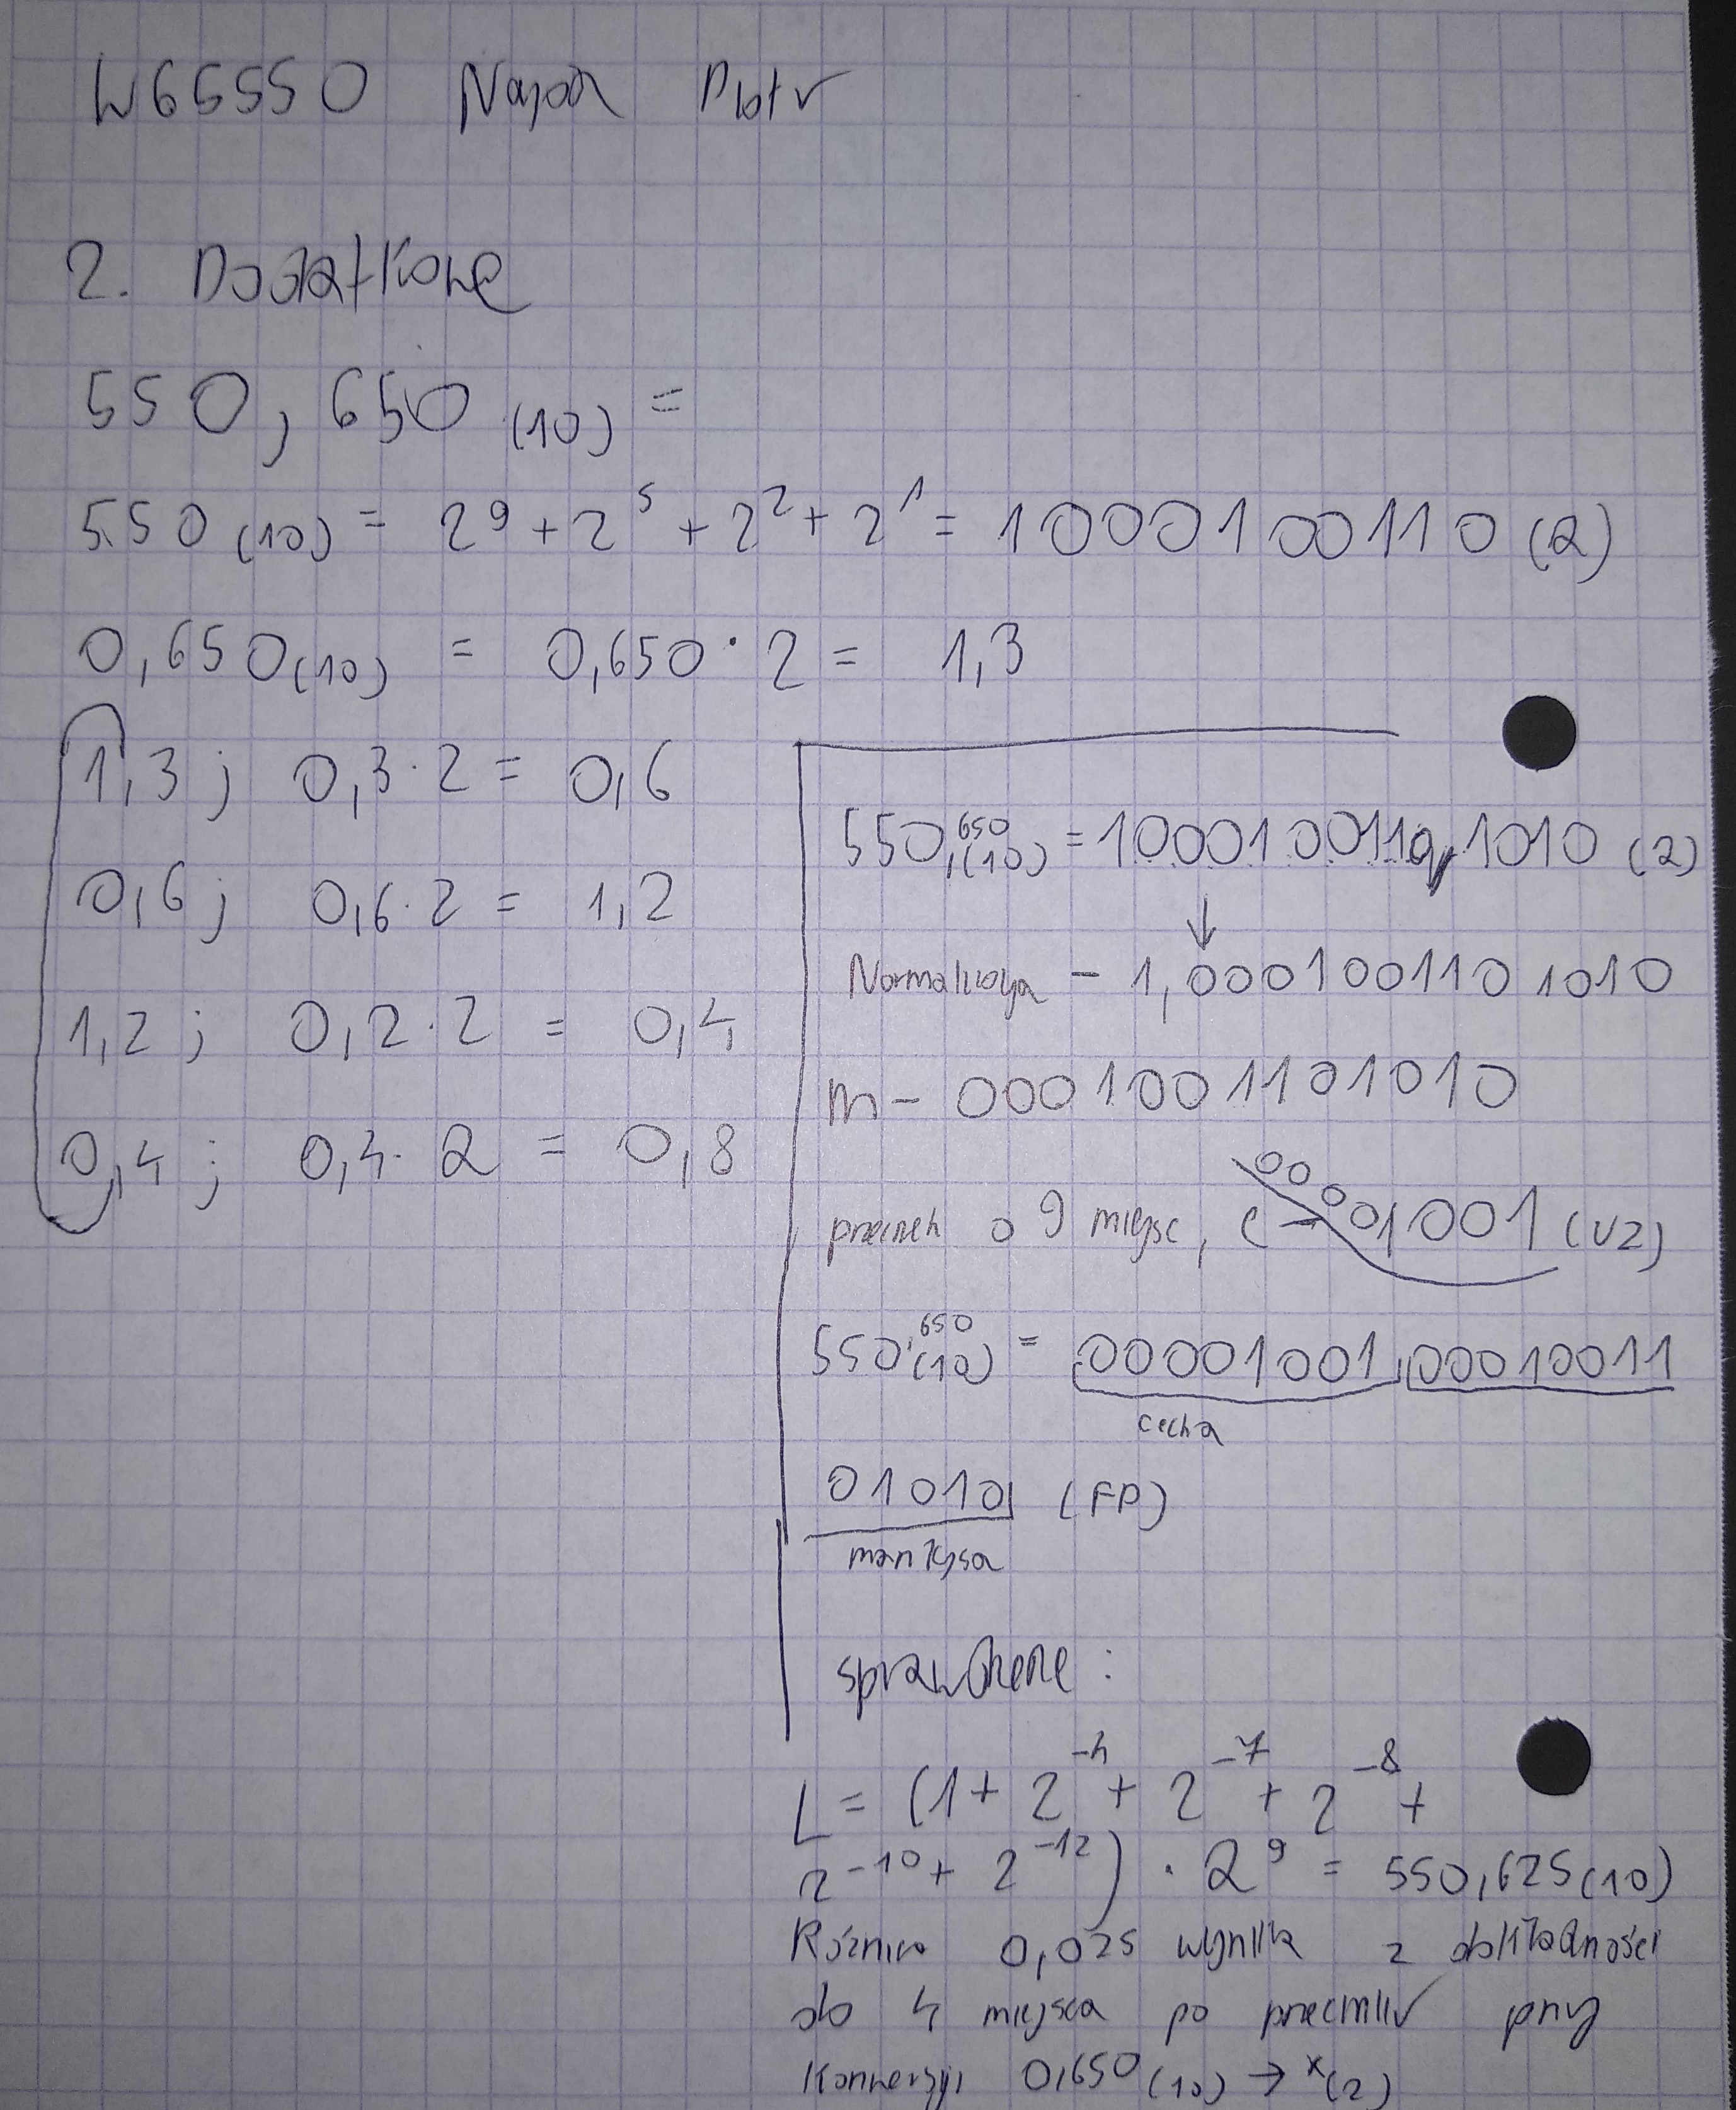
\includegraphics[width=0.9\textwidth]{IMG_20211102_174542~2.jpg}
\caption{\label{fig:zaddod2}Zadanie dodatkowe 2}
\end{figure}

\end{document}